\documentclass[11pt,letterpaper]{article}
\usepackage[lmargin=1in,rmargin=1in,bmargin=1in,tmargin=1in]{geometry}
\usepackage{checkins}

\pgfplotsset{soldot/.style={color=black,only marks,mark=*},
		holdot/.style={color=black,fill=white,only marks,mark=*},
		compat=1.12
}

% -------------------
% Content
% -------------------
\begin{document}
\thispagestyle{title}

% 08/22
\checkin{08/22} If $\ds\lim_{x \to 5} f(x)= -3$, then $f(5)= -3$. \pspace

\sol The statement is \textit{false}. A function's limit (if it even exists) \textit{does not} have to be the same as the function's value at that limiting value---the function does not even have to be defined there! Consider the three examples below. \par
	\begin{center}
	% Left
	\fbox{%
	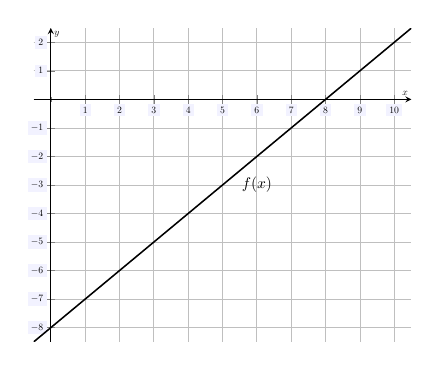
\begin{tikzpicture}[scale=0.7,every node/.style={scale=0.5}]
	\begin{axis}[
	grid=both,
	axis lines=middle,
	ticklabel style={fill=blue!5!white},
	xmin= -0.5, xmax=10.5,
	ymin= -8.5, ymax=2.5,
	xtick={-1,0,...,11},
	ytick={-8,-7,...,2},
	minor tick = {-9,-8,...,3},
	xlabel=\(x\),ylabel=\(y\),
	samples=20]
	\node at (6,-3) {\scalebox{1.6}{$f(x)$}};
	\addplot[thick, samples=5, domain= -0.5:10.5] {x - 8};
	\end{axis}
	\end{tikzpicture}
	} \hfill
	% Middle
	\fbox{%
	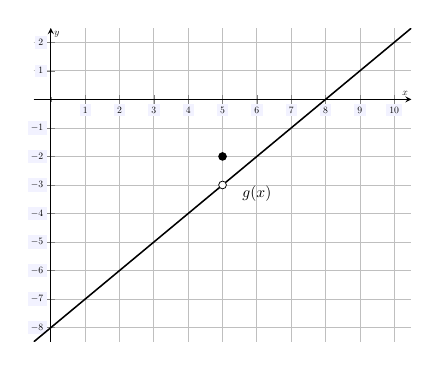
\begin{tikzpicture}[scale=0.7,every node/.style={scale=0.5}]
	\begin{axis}[
	grid=both,
	axis lines=middle,
	ticklabel style={fill=blue!5!white},
	xmin= -0.5, xmax=10.5,
	ymin= -8.5, ymax=2.5,
	xtick={-1,0,...,11},
	ytick={-8,-7,...,2},
	minor tick = {-9,-8,...,3},
	xlabel=\(x\),ylabel=\(y\),
	samples=20]
	\node at (6.0,-3.3) {\scalebox{1.6}{$g(x)$}};
	\addplot[thick, samples=5, domain= -0.5:10.5] {x - 8};
	\addplot[soldot] coordinates{(5,-2)};
	\addplot[holdot] coordinates{(5,-3)};
	\end{axis}
	\end{tikzpicture}
	} \hfill
	% Right
	\fbox{%
	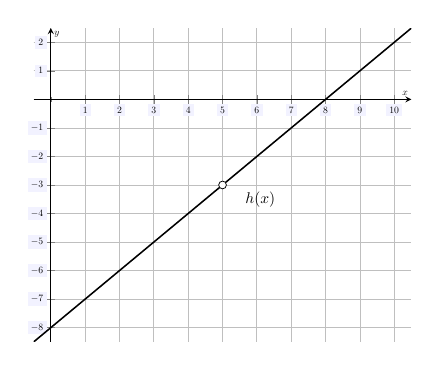
\begin{tikzpicture}[scale=0.7,every node/.style={scale=0.5}]
	\begin{axis}[
	grid=both,
	axis lines=middle,
	ticklabel style={fill=blue!5!white},
	xmin= -0.5, xmax=10.5,
	ymin= -8.5, ymax=2.5,
	xtick={-1,0,...,11},
	ytick={-8,-7,...,2},
	minor tick = {-9,-8,...,3},
	xlabel=\(x\),ylabel=\(y\),
	samples=20]
	\node at (6.1,-3.5) {\scalebox{1.6}{$h(x)$}};
	\addplot[thick, samples=5, domain= -0.5:10.5] {x - 8};
	\addplot[holdot] coordinates{(5,-3)};
	\end{axis}
	\end{tikzpicture}
	}
	\end{center} \par
For the graph of $f(x)$ on the left, $\ds\lim_{x \to 5} f(x)= -3$, so they are equal. However, observe that for $g(x)$ (the middle graph), we have $\ds\lim_{x \to 5} g(x)= -3$ but $g(5)= -2$, so that $\ds\lim_{x \to 5} g(x) \neq g(5)$. Similarly, in the graph of $h(x)$ on the right, $\ds\lim_{x \to 5} h(x)= -3$ but $h(-3)$ is not defined, so that $\ds\lim_{x \to 5} h(x) \neq h(-3)$. A function's value (if even defined) need not be related to its limit (if the limit even exists). \pvspace{1.3cm}



% 08/25
\checkin{08/25} The limit $\ds\lim_{x \to 0} \dfrac{\sin x}{x}= \text{DNE}$ because $\tfrac{\sin x}{x}$ becomes $\tfrac{0}{0}$ when one `plugs-in' $x= 0$ and $\frac{0}{0}$ is undefined. \pspace

\sol The statement is \textit{false}. In fact, $\ds\lim_{x \to 0} \dfrac{\sin x}{x}= 1$. Yes, $\tfrac{0}{0}$, $\pm\tfrac{\infty}{\infty}$, $0 \cdot \infty$, $\infty - \infty$, $0^0$, $1^\infty$, and $\infty^0$ are indeterminant/undefined expressions. However, that does not mean that the limit they arise from does not exist. The limit could exist or not---just like \textit{any} limit. `Running into' one of these expressions when evaluating a limit at its limiting value only means that one needs to try a different approach to determine if the limit exists or not. \pvspace{1.3cm}



% 08/27
\checkin{08/27} $\ds\lim_{x \to 0} \dfrac{\tan(5x)}{5x}= 1$ \pspace

\sol The statement is \textit{true}. Recall that $\ds\lim_{x \to 0} \dfrac{\sin(x)}{x}= 1$. We should think of this as $\ds\lim_{\Box \to 0} \dfrac{\sin \Box}{\Box}= 1$. But then\dots
	\[
	\lim_{x \to 0} \dfrac{\tan(5x)}{5x}= \lim_{x \to 0} \dfrac{\tfrac{\sin(5x)}{\cos(5x)}}{5x}= \lim_{x \to 0} \dfrac{\sin(5x)}{5x \cos x}= \lim_{x \to 0} \left( \dfrac{\sin(5x)}{5x} \cdot \dfrac{1}{\cos(5x)} \right)
	\]
Using the fact that $\ds\lim_{\Box \to 0} \dfrac{\sin \Box}{\Box}= 1$, we then have\dots
	\[
	\lim_{x \to 0} \dfrac{\tan(5x)}{5x}= \lim_{x \to 0} \left( \dfrac{\sin(5x)}{5x} \cdot \dfrac{1}{\cos(5x)} \right)= 1 \cdot \dfrac{1}{\cos(0)}= 1 \cdot \dfrac{1}{1}= 1
	\] \pvspace{1.3cm}



% 08/29
\checkin{08/29} $\ds\lim_{x \to 2^+} \dfrac{x - 3}{x - 2}= \infty$ \pspace

\sol The statement is \textit{false}. Observe that plugging-in $x= 2$, we obtain $\frac{-1}{0}$, which is undefined. However, this indicates that this is a `thinking limit'. Because in the limit, $x$ is `close' to 2, $x - 3$ is negative. As we approach 2 from the right, $x > 2$ so that $x - 2$ is positive. But then\dots
	\[
	\lim_{x \to 2^+} \dfrac{\overbrace{x - 3}^{-}}{\underbrace{x - 2}_{+}}= -\infty
	\] \pvspace{1.3cm}



% 09/03
\checkin{09/03} $\ds\lim_{x \to \infty} \dfrac{x^3 - 1}{1 - x^2}= -\infty$ \pspace

\sol The statement is \textit{true}. This is a rational limit. Observe that the degree of the numerator is 3 while the degree of the denominator is 2. Therefore, we know the limit will be $\pm\infty$. Observe that in the numerator, $x \to \infty$, so we know that $x^3 \to \infty$. In the denominator, we know that $x \to \infty$, so that $-x^2 \to -\infty$. Therefore, it should be that the limit tends to $-\infty$. We can confirm this intuition with the appropriate algebraic `trick': we divide the numerator and denominator by the `dominating' term in the denominator, which in this case is $x^2$:
	\[
	\lim_{x \to \infty} \dfrac{x^3 - 1}{1 - x^2}= \lim_{x \to \infty} \dfrac{x^3 - 1}{1 - x^2} \cdot \dfrac{1/x^2}{1/x^2}= \lim_{x \to \infty} \dfrac{\tfrac{x^3}{x^2} - \tfrac{1}{x^2}}{\tfrac{1}{x^2} - \tfrac{x^2}{x^2}}= \lim_{x \to \infty} \dfrac{x - \cancel{\tfrac{1}{x^2}}^{\,{}^0}}{\cancel{\tfrac{1}{x^2}}^{\,{}^0} - 1}= -\infty
	\] \pvspace{1.3cm}



% 09/05
\checkin{09/05} If $f(x)$ is a function and $\ds\lim_{x \to 1} f(x) = f(1)$, then $f(x)$ must be continuous at $x= 1$. \pspace

\sol The statement is \textit{true}. A function $f(x)$ is continuous at $x= a$ if $\ds f(a)= \lim_{x \to a} f(x)$. The statement of the problem states that $\ds\lim_{x \to 1} f(x)= f(1)$, i.e. $\ds f(1)= \lim_{x \to 1} f(x)$. Therefore, $f(x)$ is continuous at $x= 1$. Similarly, if we knew $f(x)$ was continuous at $x= 1$, then we would know that $\ds f(1)= \lim_{x \to 1} f(x)$. \pvspace{1.3cm}



% 09/07
\checkin{09/07} If $f(x)$ is given by\dots
	\[
	f(x)=
	\begin{cases}
	x + 1, & x \geq 0 \\
	4, & x < 0
	\end{cases}
	\]
Then $f(x)$ is differentiable at $x= 0$. \pspace

\sol The statement is \textit{false}. Recall that $f(x)$ is continuous at $x= a$ if $\ds f(a)= \lim_{x \to a} f(x)$ and that if a function is differentiable at $x= a$, then $f(x)$ is continuous at $x= a$. Therefore, $f(x)$ is continuous at $x= 0$ if and only if $\ds f(0)= \lim_{x \to 0} f(x)$. Observe that $f(0)= 0 + 1= 1$, $\ds\lim_{x \to 0^-} f(x)= \lim_{x \to 0^-} 4= 4$, and $\ds\lim_{x \to 0^+} f(x)= \lim_{x \to 0^+} (x + 1)= 0 + 1= 1$. Because $\ds\lim_{x \to 0^-} f(x) \neq \lim_{x \to 0^+} f(x)$, i.e. the left and right hand limits are not equal, $\ds\lim_{x \to 0} f(x)$ does not exist. But then $f(0) \neq \lim_{x \to 0} f(x)$, so that $f(x)$ is not continuous at $x= 0$. Because $f(x)$ is not continuous at $x= 0$, $f(x)$ cannot be differentiable at $x= 0$. \pspace

We can also verify this directly from the definition of the derivative. Recall that $\ds f'(a):= \lim_{h \to 0} \dfrac{f(a + h) - f(a)}{h}$. Here, we have $a= 0$ and $f(0)= 0 + 1= 1$. We compute this limit by computing the left and right hand limits. We have\dots
	\[
	\begin{aligned}
	\lim_{h \to 0^-} \dfrac{f(0 + h) - f(0)}{h}= \lim_{h \to 0^-} \dfrac{f(h) - f(0)}{h}= \lim_{h \to 0^-} \dfrac{4 - 1}{h}= \lim_{h \to 0^-} \dfrac{3}{h}= -\infty \\[0.3cm]
	\lim_{h \to 0^+} \dfrac{f(0 + h) - f(0)}{h}= \lim_{h \to 0^+} \dfrac{f(h) - f(0)}{h}= \lim_{h \to 0^+} \dfrac{(h + 1) - 1}{h}= \lim_{h \to 0^+} 1= 1 \\
	\end{aligned}
	\]
Because $\ds \lim_{h \to 0} \dfrac{f(0 + h) - f(0)}{h}$ does not exist, $f'(0)$ does not exist, i.e. $f(x)$ is not differentiable at $x= 0$. \pvspace{1.3cm}



% 09/10
\checkin{09/10} $\dfrac{d}{dx} \left( e^{\sin x} \right)= e^{\cos x}$ \pspace

\sol The statement is \textit{false}. Observe that the given solution, $e^{\cos x}$, has the derivative of both $e^x$ (which is $e^x$) and $\sin x$ (which is $\cos x$) simultaneously. However, all the derivative rules only ever have one taking the derivative of \textit{one} function at a time for any corresponding term. If we choose $f(x)= e^x$ and $g(x)= \sin x$, we have $f \big( g(x) \big)= f(\sin x)= e^{\sin x}$. We know that $f'(x)= e^x$ and $g'(x)= \cos x$. Using the chain rule, $\tfrac{d}{dx} f \big( g(x) \big)= f' \big( g(x) \big) \cdot g'(x)$, we have $\tfrac{d}{dx} e^{\sin x}= e^{\sin x} \cdot \cos x= e^{\sin x} \cos x$. Alternatively, using the `box method' or `onion approach', the first `layer' is $e^\Box{}$, whose derivative is $e^\Box{}$. We multiply by the derivative of the contents of $\Box{}$, which is the derivative of $\sin x$, i.e. $\cos x$. But then the derivative is $e^{\sin x} \cos x$. \pvspace{1.3cm}



% 09/11
\checkin{09/11} $\dfrac{d}{dx} \,\left( x^4 \csc(x) e^x \right)= 4x^3 \cdot \csc(x) e^x + -\csc x \cot x \cdot x^4 e^x + e^x \cdot x^4 \csc x$ \pspace

\sol The statement is \textit{true}. Although we can use the Product Rule: $\dfrac{d}{dx} (fg)= f'g + fg'$, it is simpler to recall that the Product Rule is a `one at a time rule.' That is, the product rule says to add together the product of the terms where the derivative of only one of the terms has been taken. Using this approach, we have\dots
	\[
	\begin{aligned}
	\dfrac{d}{dx} \,\left( x^4 \csc(x) e^x \right)&= \dfrac{d}{dx} (x^4) \cdot \csc x e^x + \dfrac{d}{dx} (\csc x) \cdot x^4 e^x + \dfrac{d}{dx}(e^x) \cdot x^4 \csc x \\[0.3cm]
	&= 4x^3 \cdot \csc(x) e^x + -\csc x \cot x \cdot x^4 e^x + e^x \cdot x^4 \csc x
	\end{aligned}
	\] \pvspace{1.3cm}



% 09/15
\checkin{09/15} $\dfrac{d}{dx} \left( \dfrac{x^2}{4x - 3} \right)= \dfrac{4(x^2) - 2x(4x - 3)}{(4x - 3)^2}$ \pspace

\sol The statement is \textit{false}. Recall that the quotient rule is given by $\frac{d}{dx} \left( \frac{f}{g} \right)= \frac{f' g - g' f}{g^2}$, i.e. the derivative of the bottom `gets the negative for its derivative' or the `\textbf{\underline{n}}umerator function' gets the \textbf{\underline{n}}egative. Observe that the given solution has the order of subtraction in the numerator reversed, i.e. it is the negative of the correct answer; that is, the numerator is `backwards' from the actual quotient rule. The correct answer should be:
	\[
	\dfrac{d}{dx} \left( \dfrac{x^2}{4x - 3} \right)= \dfrac{2x(4x - 3) - 4(x^2)}{(4x - 3)^2}
	\] \pvspace{1.3cm}



% 09/17
\checkin{09/17} If $f(x)$ is a function with $f(1)= 3$ and $f'(1)= 10$, then it should be that $f(0.8) \approx 1$. \pspace

\sol The statement is \textit{true}. The linearization of $f(x)$ at $x= a$ is $\ell_a(x)= f(a) + f'(a) \,\big( x - a \big)$. We know that if $x$ is `close' to $a$, then $f(x) \approx \ell_a(x)$. The linearization of the given $f(x)$ at $x= 1$ is $\ell_1(x)= f(1) + f'(1) \,\big( x - 1 \big)= 3 + 10(x - 1)$. But then we have\dots
	\[
	f(0.8) \approx \ell_1(0.8)= 3 + 10(0.8 - 1)= 3 + 10(-0.2)= 3 + (-2)= 1
	\] \pvspace{1.3cm}



% 09/24
\checkin{09/24} The critical value(s) for $f(x)= 2x + \frac{1}{x^2}$ is $x= 1$. \pspace

\sol The statement is \textit{false}. Recall the critical value(s) for a function $f(x)$ are the value(s) for which $f'(x)$ is 0 or undefined. Because $f(x)= 2x + \frac{1}{x^2}= 2x + x^{-2}$, we have $f'(x)= 2 - 2x^{-3}= 2 - \frac{2}{x^3}$. Observe that $f'(x)$ is undefined at $x= 0$, so that $x= 0$ is a critical value. Solving $f'(x)= 0$, we have\dots
	\[
	\begin{gathered}
	f'(x)= 0 \\
	2 - \frac{2}{x^3}= 0 \\
	2= \frac{2}{x^3} \\
	2x^3= 2 \\
	x^3= 1 \\
	x= 1
	\end{gathered}
	\]
Therefore, $x= 1$ is a critical value. Therefore, the critical values are $x= 0, 1$. \pvspace{1.3cm}



% 09/26
\checkin{09/26} $\ds\lim_{x \to 0} \dfrac{\sin(4x)}{5x} \stackrel{\text{LH}}{=} \lim_{x \to 0} \dfrac{4\cos(4x)}{5}= \dfrac{4}{5}$ \pspace

\sol The statement is \textit{true}. Na\"ively evaluating the argument at $x= 0$, we obtain $\frac{0}{0}$. But then l'H\^{o}pital's should apply. The derivative of $\sin(4x)$ is $\cos(4x) \cdot 4= 4 \cos(4x)$ and the derivative of $5x$ is $5$. But then\dots
	\[
	\lim_{x \to 0} \dfrac{\sin(4x)}{5x} \stackrel{\text{LH}}{=} \lim_{x \to 0} \dfrac{4\cos(4x)}{5}= \dfrac{4 \cos(0)}{5}= \dfrac{4(1)}{5}= \dfrac{4}{5}
	\]
However, we can also recognize this as a `special limit', $\ds\lim_{\Box{} \to 0} \dfrac{\sin \Box{}}{\Box{}}= 1$, and solve it this way:
	\[
	\lim_{x \to 0} \dfrac{\sin(4x)}{5x}= \lim_{x \to 0} \dfrac{1}{5} \dfrac{\sin(4x)}{x}= \lim_{x \to 0} \dfrac{1}{5} \dfrac{\sin(4x)}{4x} \cdot 4= \dfrac{1}{5} \cdot 1 \cdot 4= \dfrac{4}{5}
	\] \pvspace{1.3cm}



% 09/29
\checkin{09/29} $\ds\lim_{x \to 1} \dfrac{3x^2 - 2x - 1}{x^2 - 2x + 1} \stackrel{\text{L.H.}}{=} \lim_{x \to 1} \dfrac{6x - 2}{2x - 2} \stackrel{\text{L.H.}}{=} \dfrac{6}{2}= 3$ \pspace

\sol The statement is \textit{false}. Na\"ively plugging in $x= 1$ into $\dfrac{3x^2 - 2x - 1}{x^2 - 2x + 1}$, we obtain $\frac{0}{0}$, so l'H\^{o}pital's rule applies. Applying l'H\^{o}pital's rule, we obtain $\ds\lim_{x \to 1} \dfrac{6x - 2}{2x - 2}$. However, now na\"ively plugging in $x= 1$, we obtain $\frac{4}{0}$ and l'H\^{o}pital's rule does not apply. Indeed, this is now a `thinking limit.' One can show that this limit does not exist. [In fact, this shows the initial application does not necessarily hold. However, $\dfrac{3x^2 - 2x - 1}{x^2 - 2x + 1}= \dfrac{(3x + 1)(x - 1)}{(x - 1)^2}$. But then $\ds\lim_{x \to 1} \dfrac{3x^2 - 2x - 1}{x^2 - 2x + 1}= \lim_{x \to 1} \dfrac{3x + 1}{x - 1}$ and this limit does not exist.] \pvspace{1.3cm}



% 10/01
\checkin{10/01} $\ds\lim_{x \to 0^+} \left( \dfrac{1}{\sin x} - \dfrac{1}{x} \right) \stackrel{\text{L.H.}}{=} \lim_{x \to 0^+} \left( \dfrac{1}{\cos x} - \dfrac{1}{1} \right)$ \pspace

\sol The statement is \textit{false}. Observe that if one na\"ively evaluates $\dfrac{1}{\sin x} - \dfrac{1}{x}$ at $x= 0$, one obtains $\infty - \infty$, which is indeterminant. However, we recognize this as a limit to which l'H\^opital's will typically be applied to. However, l'H\^opital's rule does not immediately apply as it can only be used in the case of the indeterminant forms $\frac{0}{0}$ or $\pm \frac{\infty}{\infty}$. Even if l'H\^opital's rule could be applied, recall that it says that if $\ds\lim \frac{f}{g}$ is $\frac{0}{0}$ or $\pm \frac{\infty}{\infty}$, then $\ds\lim \frac{f}{g}= \lim \frac{f'}{g'}$ (so long as $\ds\lim \frac{f'}{g'}$ exists). So, even if l'H\^opital's rule applied, it would have not been applied correctly here because there was not a single fraction and `l'H\^opital's was applied' to only the denominators of the separate fractions. \pspace

In the case of the indeterminant form $\infty - \infty$, we often factor a term out or combine terms. In this case, creating a common denominator, we have\dots
	\[
	\lim_{x \to 0^+} \left( \dfrac{1}{\sin x} - \dfrac{1}{x} \right)= \lim_{x \to 0^+} \dfrac{x - \sin x}{x \sin x}
	\]
Observe that now na\"ively evaluating $\dfrac{x - \sin x}{x \sin x}$ at $x= 0$, one obtains $\frac{0}{0}$. But then l'H\^opital's rule applies. So, we have\dots
	\[
	\lim_{x \to 0^+} \dfrac{x - \sin x}{x \sin x} \stackrel{\text{L.H.}}{=} \lim_{x \to 0^+} \dfrac{1 - \cos x}{\sin x + x \cos x}
	\]
Na\"ively evaluating $\dfrac{1 - \cos x}{\sin x + x \cos x}$ at $x= 0$, we obtain $\frac{0}{0}$. So, we use l'H\^opital's again: 
	\[
	\lim_{x \to 0^+} \dfrac{1 - \cos x}{\sin x + x \cos x} \stackrel{\text{L.H.}}{=} \lim_{x \to 0^+} \dfrac{\sin x}{\cos x + (\cos x - x \sin x)}= \lim_{x \to 0^+} \dfrac{\sin x}{2 \cos x - x \sin x}= \dfrac{0}{2(1) - 0}= 0
	\]
Therefore, $\\lim_{x \to 0^+} \left( \dfrac{1}{\sin x} - \dfrac{1}{x} \right)= 0$. \pvspace{1.3cm}



% 10/03
\checkin{10/03} $\dfrac{d}{dt} \left( x \sin(xy) \right)= x' \sin(xy) + x \cos(xy) \big(x' y + y' x)$ \pspace

\sol The statement is \textit{true}. If $x, y$ do not depend on $t$, then clearly $\dfrac{d}{dt} \left( x \sin(xy) \right)= 0$. However, if we do not know this to be the case, we can always implicitly differentiate, which will give us a correct answer regardless of whether $x, y$ depends on $t$. Assuming $x, y$ might depend on $t$, observe that $x \sin(xy)$ is a product of functions which depend on $t$. So, we need a product rule (which will also require a chain rule for the term $\sin(xy)$):
	\[
	\begin{aligned}
	\dfrac{d}{dt} \left( x \sin(xy) \right)&= \dfrac{d}{dt}(x) \cdot \sin(xy) + x \cdot \dfrac{d}{dt} \big( \sin(xy) \big) \\
	&= \frac{dx}{dt}\, \sin(xy) + x \cos(xy) \cdot \dfrac{d}{dt} (xy) \\
	&= \frac{dx}{dt}\, \sin(xy) + x \cos(xy) \cdot \left( \dfrac{d}{dt}(x) \cdot y + x \cdot \dfrac{d}{dt}(y) \right) \\
	&= \frac{dx}{dt}\, \sin(xy) + x \cos(xy) \cdot \left( \dfrac{dx}{dt}(x) \cdot y + x \cdot \dfrac{dy}{dt} \right) \\
	&= x' \sin(xy) + x \cos(xy) \,(x' y+ y' x)
	\end{aligned}
	\] \pvspace{1.3cm}



% 10/06
\checkin{10/06} One can substitute anything that is constant throughout the problem into the equation to be differentiated in a related rates problem without introducing an error. \pspace

\sol The statement is \textit{true}. This is easiest seen in an example. Suppose we had a problem where the side lengths of a right triangle were changing in time but one side was constant. Say that $a, b$ and $c$ were the legs and hypotenuse of the triangle, respectively, and that $a, c$ were changing in time but $b$ was not. We know that $a^2 + b^2= c^2$. Because $b$ is constant with respect to time, we could substitute it before differentiating with respect to time. Say that $b= 5$. We would then have\dots
	\[
	\begin{gathered}
	a^2 + b^2= c^2 \\
	a^2 + 5^2= c^2 \\
	\dfrac{d}{dt} \,(a^2 + 5^2)= \dfrac{d}{dt} \,c^2 \\
	2aa' + 0= 2cc' \\
	2aa'= 2cc' \\
	aa'= cc'
	\end{gathered}
	\]
We did not \textit{have} to substitute this $b$-value. If we had not, we would have\dots
	\[
	\begin{gathered}
	a^2 + b^2= c^2 \\
	\dfrac{d}{dt} \,(a^2 + b^2)= \dfrac{d}{dt} \,c^2 \\
	2aa' + 2bb'= 2cc' \\
	aa' + bb'= cc'
	\end{gathered}
	\]
Why is the same as the original answer above? If $b$ is constant with respect to time, then $b'= 0$ because $b$ is not changing. But then\dots
	\[
	\begin{gathered}
	aa' + bb'= cc' \\
	aa' + b(0)= cc' \\
	aa'= cc' 
	\end{gathered}
	\]
However, suppose that $b$ was \textit{not} constant with respect to time but we still had $b= 5$ at some moment in time. If we substituted it as above, we would obtain the same result as we did in the original answer, $aa'= cc'$, where we should have obtained $aa' + bb'= cc'$ as we did in the second answer. So, in a related rates problem, one can only substitute values which are constant with respect to the differentiated variable before differentiating. \pvspace{1.3cm}



% 010/08
\checkin{10/08} $\dfrac{d}{dx}\,(y^2 \cdot y')= 2y \cdot y' + y^2 \cdot y''$ \pspace

\sol The statement is \textit{false}. The answer given in the problem statement has missed the $y'$ term produced by differentiating $y^2$ implicitly---likely because of the $y'$ term already present. We have\dots
	\[
	\dfrac{d}{dx}\,(y^2 \cdot y')= \dfrac{d}{dx}(y^2) \cdot y' + y^2 \cdot \dfrac{d}{dx}(y')= (2yy') \cdot y' + y^2 \cdot y''= 2y (y')^2 + y^2 \cdot y''
	\] \pvspace{1.3cm}



% 010/13
\checkin{10/13} It is often easier to work with the square of the distance between two points rather than the distance itself, and this approach will often yield the same answer in the end. \pspace

\sol The statement is \textit{true}. Although this is not necessarily universally true, this is often the case. Consider the example when we want to determine how the distance from a point $(x, y)$ to the point $(1, -2)$ changes in time. The distance is $d= \sqrt{(x - 1)^2 + \big(y - (-2) \big)^2}= \sqrt{(x - 1)^2 + (y + 2)^2}$. Then the rate of change of this distance in time is\dots
	\[
	d'= \dfrac{d}{dt}\, \sqrt{(x - 1)^2 + \big(y - (-2) \big)^2}= \dfrac{2(x - 1) x' + 2(y + 2) y'}{2 \sqrt{(x - 1)^2 + \big(y + 2 \big)^2}}= \dfrac{(x - 1) x' + (y + 2) y'}{\sqrt{(x - 1)^2 + \big(y + 2 \big)^2}}
	\]
Although this derivative is not necessarily that difficult, it is tedious. Compare to this to workin with $d^2= (x - 1)^2 + (y + 2)^2$. Differentiating in time, we have\dots
	\[
	\begin{gathered}
	\dfrac{d}{dt}\, d^2= \dfrac{d}{dt}\, \left[ (x - 1)^2 + (y + 2)^2 \right] \\
	2dd'= 2(x - 1) x' + 2(y + 2) y' \\
	dd'= (x - 1) x' + (y + 2) y'
	\end{gathered}
	\]
This is just as easy to find $d'$ for---perhaps easier---given $x, y, x', y'$ than the expression we found before. We can even find the same equation as above. We know that $d= \sqrt{(x - 1)^2 + (y + 2)^2}$. But then\dots
	\[
	\begin{gathered}
	dd'= (x - 1) x' + (y + 2) y' \\
	d'= \dfrac{(x - 1) x' + (y + 2) y'}{d} \\
	d'= \dfrac{(x - 1) x' + (y + 2) y'}{\sqrt{(x - 1)^2 + (y + 2)^2}}
	\end{gathered}
	\]
This same strategy will also be useful for optimization as well. \pvspace{1.3cm}



% 010/15
\checkin{10/15} If $x_0$ is a local minimum for $d^2= (x - 1)^2 + \big( f(x) + 4 \big)^2$, then it is a minimum for $d= \sqrt{(x - 1)^2 + \big( f(x) + 4 \big)^2}$. \pspace

\sol The statement is \textit{true}. The distance between a point on a function, $f(x)$, i.e. $\big(x, f(x) \big)$, and a point $(1, -4)$ is given by\dots
	\[
	d= \sqrt{(x_1 - x_2)^2 + (y_1 - y_2)^2}= \sqrt{(x - 1)^2 + \big(f(x) - (-4) \big)^2}= \sqrt{(x - 1)^2 + \big(f(x) + 4 \big)^2}
	\]
While minimizing/maximizing $d^2$ instead of $d$ may result in different minimum/maximum \textit{values}, the location of these minimum/maximum values remains the same. That is, $d^2$ and $d$ have the same critical values. So, instead of minimizing/maximizing $d$, we can minimize/maximize $d^2$, which is simpler to work with because of the lack of square root, c.f. the previous check-in. \pvspace{1.3cm}



% 10/17
\checkin{10/17} The area of an equilateral triangle with side length $s$ is $\frac{\sqrt{3}}{4}\, s^2$. \pspace

\sol The statement is \textit{true}\dots there's not much else to say. \pvspace{1.1cm}



% 10/29
\checkin{10/29} Let $f(x)= \dfrac{2x + 5}{x - 3}$. Observe that $f(2)= -9$ and $f(4)= 13$, $-9 < 0 < 13$, and $-9 < 2 < 13$. By the Intermediate Value Theorem, there exists $c_1 \in [2, 4]$ such that $f(c_1)= 0$ and there also exists $c_2 \in [2, 4]$ such that $f(c_2)= 2$. \pspace

\sol The statement is \textit{false}. Recall that the Intermediate Value Theorem (IVT) states the following: if $f(x)$ is continuous on $[a, b]$ and $y$ is between $f(a)$ and $f(b)$, there exists $c \in [a, b]$ such that $f(c)= y$; that is, if a continuous function takes on two different values on an interval, it takes on every value between those values at some point on the interval. But the function needs to be continuous. Observe that the given $f(x)$ is not continuous at $x= 3$---it is not even defined there. So, $f(x)$ is not continuous on $[2, 4]$ because $3 \in [2, 4]$. In fact, there is a $x$-value such that $f(x)= 0$, namely $x= -\frac{5}{2}$ but this value is not in $[2, 4]$. While it is true that $-9 < 2 < 13$, the IVT does not apply because $f(x)$ is not continuous on $[2, 4]$. Furthermore, there is no $x$-value such that $f(x)= 2$. If there were, then $\frac{2x + 5}{x - 3}= 2$. Multiplying by $x - 3$ (so long as $x \neq 3$), we have $2x + 5= 2x - 6$, which implies that $5= -6$, which is impossible. In fact, $y= 2$ is a horizontal asymptote for $f(x)$ as $\ds\lim_{x \to \pm \infty} f(x)= 2$. \pvspace{0.8cm}



% 10/31
\checkin{10/31} If 30 people enter a room over 5 hours, then there was an hour where \textit{at least} 6 people entered the room but not necessarily an hour where \textit{exactly} 6 people entered the room. \pspace

\sol The statement is \textit{true}. Recall that the Mean Value Theorem (MVT) states the following: if $f(x)$ is continuous on $[a, b]$ and differentiable on $(a, b)$, then there exists $c \in (a, b)$ such that $f'(c)= \frac{f(b) - f(a)}{b - a}$; that is, if $f(x)$ is continuous on $[a, b]$ and differentiable on $(a, b)$, then there is at least one point on the interval $(a, b)$ where the instantaneous rate of change is the average rate of change, i.e. the slope of the tangent line is parallel to the line through the endpoints of the function on the interval. Let $f(x)$ be the number of people that have entered the room $x$~hours from now. We know $f(0)= 0$ and $f(5)= 30$. The average rate of change is $\frac{f(5) - f(0)}{5 - 0}= \frac{30}{5}= 6$. However, the MVT does not apply because the function $f(x)$ is not continuous (and hence not differentiable) on $[0, 5]$. Observe that $f(x)$ is a step function---it changes by integer values. For instance, if a person enters 2 hours from now, $f(2)= 1$. But $f(x)= 0$ for $x < 2$, so that $f(x)$ has a jump discontinuity at $x= 2$. It could be that 30 people entered the room at the fifth hour. So, there need not be an hour where \textit{exactly} 6 people entered the room. However, there must be an hour where \textit{at least} 6 people entered the room. If not, then every hour 5 or less people entered the room. But then after 5 hours, at most $5 \cdot 5= 25$ people entered the room, contradicting the fact that 30~people entered the room. The fact that there must be an hour where \textit{at least} 6 people entered the room is a consequence of the `discrete version' of the MVT---the Pigeonhole Principle: if there are $n$ items placed into $m$ containers with $n > m$, then at least one container must contain more than one item. \pvspace{1.3cm}



% 11/03
\checkin{11/03} $\ds\int_a^b c \;dx= c(b - a)$ \pspace

\sol The statement is \textit{true}. Recall that the definite integral $\ds\int_a^b f(x) \;dx$ is the area `under' the curve $f(x)$ (area between the curve $f(x)$ and the $x$-axis) between $x= a$ and $x= b$, where area under the $x$-axis is treated as `negative area.' We have $f(x)= c$, whose graph is a horizontal line. But then $\ds\int_a^b f(x) \;dx$ is the area of a rectangle with area $A= \ell w= c(b - a)$. Therefore, $\ds\int_a^b f(x) \;dx= c(b -a)$. \par
	\[
	\fbox{%
	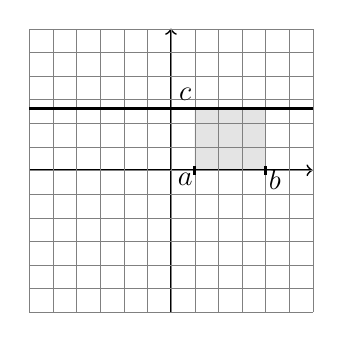
\begin{tikzpicture}[scale=0.6,every node/.style={scale=0.5}]
	\draw[draw=none,fill=gray!30,opacity=0.7] (0.5,0) -- (0.5,1.3) -- (2,1.3) -- (2,0) -- (0.5,0);
	\draw[line width=0.022cm,->] (0,-3) -- (0,3);
	\draw[line width=0.022cm,->] (-3,0) -- (3,0);
	\foreach \x in {-3,-2.5,...,3} {
		\draw[line width=0.01,gray] (\x,-3) -- (\x,3);
		\draw[line width=0.01,gray] (-3,\x) -- (3,\x);
	};
	\draw[line width=0.04cm] (-3,1.3) -- (3,1.3);
	\draw[line width=0.04cm] (0.5,-0.1) -- (0.5,0.1);
	\draw[line width=0.04cm] (2,-0.1) -- (2,0.1);
	\node at (0.3,1.6) {\huge$c$};
	\node at (0.3,-0.2) {\huge$a$};
	\node at (2.2,-0.2) {\huge$b$};
	\end{tikzpicture}
	}
	\]
Alternatively, we can use the Fundamental Theorem of Calculus to compute the integral:
	\[
	\int_a^b c \;dx= cx \bigg|_{x=a}^{x=b}= c(b - a)
	\] \pvspace{1.3cm}



% 11/05
\checkin{11/05} If $f(x)$ is a differentiable function on $[a, b]$, then $\ds\int_a^b f'(x) \;dx$ gives the net change of $f(x)$ on the interval $[a, b]$. \pspace

\sol The statement is \textit{true}. We know that $f'(x)$ gives the instantaneous rate of change of $f(x)$ at $x$. If the integral exists, we know that $\ds\int_a^b f'(x) \;dx$ is the limit---for example---of the left-hand sums. Simply put, the area of each box in the left-hand sum is a small amount of change in $f(x)$ because the width of each box is a $\Delta x$ and the height of each box is $f'(x)$. But then $A= f'(x) \Delta x= \Delta f$. Summing all these areas then sums the small amount of change in $f(x)$ at each $x$---finding the total change in $f(x)$. So, $\ds\int_a^b f'(x) \;dx$ computes the net change in $f(x)$ over $[a, b]$. \pspace

Formally, if we use an approximation to the integral with $n$ rectangles (say a left-hand sum), the width of each rectangle is $\Delta x= \frac{b - a}{n}$. The $x$-values we use are $x_i= a + i \,\Delta x= a + i \cdot \frac{b - a}{n}$. So, the height of each rectangle is given by $f'(x_i)= f \left( a + i \cdot \frac{b - a}{n} \right)$. Each rectangle then has area $A_i= \ell w= f' \left( a + i \cdot \frac{b - a}{n} \right) \cdot \Delta x$. But then\dots
	\[
	\ds\int_a^b f'(x) \;dx:= \lim_{n \to \infty} \sum_{i=0}^{n-1} A_i= \lim_{n \to \infty} \sum_{i=0}^{n-1} f' \left( a + i \cdot \frac{b - a}{n} \right) \Delta x_i
	\]
It follows immediately from the differentiability of $f$ that $f \left( a + i \cdot \frac{b - a}{n} \right) - f(a) \approx f' \left( a + i \cdot \frac{b - a}{n} \right) \Delta x_i$; that is, $f' \left( a + i \cdot \frac{b - a}{n} \right) \Delta x_i$ is the change in $x$ from $x= a$ to $x= a + i \cdot \frac{b - a}{n}$. But then $A_i$ represents the approximate net change in $f(x)$ from $x= a$ to $x= a + i \cdot \frac{b - a}{n}$. Summing over all these rectangles and taking the limit, we see that we have summed the changes in $f(x)$ from $x= a$ to $x= b$. Therefore, $\ds\int_a^b f'(x) \;dx:= \lim_{n \to \infty} \sum_{i=0}^{n-1} A_i$ is the net change in $f(x)$. \pvspace{1.3cm}



% 11/07
\checkin{11/07} $\ds\int (5 - \sin x + e^x) \;dx= 5x + \cos x + e^x$ \pspace

\sol The statement is \textit{false}. Recall that the indefinite integral $\ds\int f(x) \;dx$ asks the question: ``What is the most general function whose derivative is $f(x)$?'' That is, $\ds\int f(x) \;dx$ is the most general antiderivative for $f(x)$. If $F(x)$ is an antiderivative for $f(x)$, i.e. $F'(x)= f(x)$, then $\ds\int f(x) \;dx= F(x) + C$---but the `$+C$' is necessary. Antiderivatives are only unique up to a constant. The given solution is missing the `$+C$.' We should have\dots
	\[
	\int (5 - \sin x + e^x) \;dx= 5x + \cos x + e^x + C
	\] \pvspace{1.3cm}



\newpage



% 11/10
\checkin{11/10} Both $9 - \cos^2 x$ and $\dfrac{1 - \cos(2x)}{2}$ are antiderivatives for $\sin(2x)$. Therefore, $\ds\int \sin(2x) \;dx= (9 - \cos^2 x) + C$ and $\ds\int \sin(2x) \;dx= \dfrac{1 - \cos(2x)}{2} + C$. \pspace

\sol The statement is \textit{true}. Recall that a function $F(x)$ is an antiderivative for $f(x)$ if $F'(x)= f(x)$. So, we only need to prove that the derivative of the given functions is $\sin(2x)$. Making use of the identity $\sin(2x)= 2 \sin x \cos x$, observe that\dots
	\[
	\begin{aligned}
	\dfrac{d}{dx} (9 - \cos^2 x)&= 0 - 2 \cos x \cdot -\sin x= 2 \sin x \cos x= \sin(2x) \\[0.3cm]
	\dfrac{d}{dx} \left( \dfrac{1 - \cos(2x)}{2} \right)&= 0 - \dfrac{-\sin(2x)}{2} \cdot 2= \sin(2x)
	\end{aligned}
	\]
Therefore, they are both antiderivatives for $\sin(2x)$. This implies that\dots
	\[
	\begin{aligned}
	\int \sin(2x) \;dx&= (9 - \cos^2 x) + C \\[0.3cm]
	\int \sin(2x) \;dx&= \dfrac{1 - \cos(2x)}{2} + C
	\end{aligned}
	\]
Because antiderivatives are unique up to a constant, this implies that $9 - \cos^2 x$ and $\dfrac{1 - \cos(2x)}{2}$ only differ by a constant. Using the identities $\sin(2x)= \frac{1 - \cos(2x)}{2}$ and $\sin^2(x) + \cos^2(x)= 1$ (so that $\sin^2 x= 1 - \cos^2 x$), observe that\dots
	\[
	8 + \dfrac{1 - \cos(2x)}{2}= 8 + \sin^2 x= 8 + (1 - \cos^2 x)= 9 - \cos^2 x
	\] \pvspace{1.3cm}



% 11/12
\checkin{11/12} Suppose two curves $f(x)$ and $g(x)$ intersect only at $x= a$ and $x= b$. The area between them is \textit{always} then given by $\ds\int_a^b |f(x) - g(x)| \;dx$. \pspace

\sol The statement is \textit{true}. If $f(x)$ and $g(x)$ intersect only at $x= a$ and $x= b$, the region `between', i.e. bound by, the curves is precisely on the interval $[a, b]$. Intuitively, we want to be sure that the difference is taken in an order so that the difference is nonnegative---forcing the area to be nonnegative. That is, we want to be sure that the integrand is ``top minus bottom.'' However, taking the absolute value forces the value of the difference to be nonnegative---taking care of this problem for us. Rigorously, if $f(x) \geq g(x)$ on $[a, b]$, the area would be given by $\ds\int_a^b f(x) - g(x) \;dx$. But if $f(x) \geq g(x)$, then $f(x) - g(x) \geq 0$ so that $|f(x) - g(x)|= f(x) - g(x)$. But then $\ds\int_a^b |f(x) - g(x)| \;dx= \int_a^b f(x) - g(x) \;dx$. If $g(x) \geq f(x)$ on $[a, b]$, the area would be given by $\ds\int_a^b g(x) - f(x) \;dx$. But if $g(x) \geq f(x)$, then $g(x) - f(x) \geq 0$, i.e. $f(x) - g(x) \leq 0$ so that $|f(x) - g(x)|= -\big( f(x) - g(x) \big)= g(x) - f(x)$. But then $\ds\int_a^b |f(x) - g(x)| \;dx= \int_a^b g(x) - f(x) \;dx$. Therefore, the area is always given by $\ds\int_a^b |f(x) - g(x)| \;dx$. \pvspace{1.3cm}



% 11/14
\checkin{11/14} If $\ds\int_a^b \big( f(x) - g(x) \big) \;dx= -5$, then the area between $f(x)$ and $g(x)$ is $5$. \pspace

\sol The statement is \textit{false}. When finding area between curves, we know that the area must be nonnegative. Certainly, an answer of $-5$ would be incorrect. Many would say when you get a negative, one must have simply done ``bottom minus top'' instead, so that the correct answer must be the negative of what was obtained. However, the error may not be that simple. For instance, consider the example below with $f(x)$ the piecewise function shown ($1$ for $0 \leq x \leq 1$ and $-1$ for $x > 1$) and $g(x)= 0$. \par
	\[
	\fbox{%
	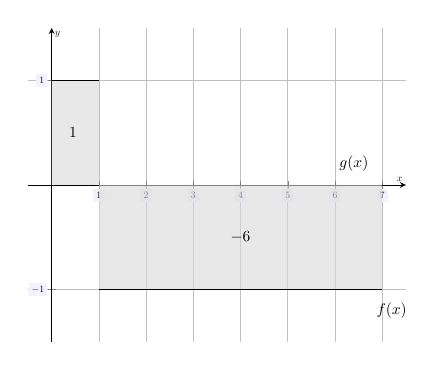
\begin{tikzpicture}[scale=0.7,every node/.style={scale=0.5}]
	\begin{axis}[
	grid=both,
	axis lines=middle,
	ticklabel style={fill=blue!5!white},
	xmin= -0.5, xmax=7.5,
	ymin= -1.5, ymax=1.5,
	xtick={-1,0,...,11},
	ytick={-8,-7,...,2},
	minor tick = {-9,-8,...,3},
	xlabel=\(x\),ylabel=\(y\),
	samples=20]
	\node at (7.2,-1.2) {\scalebox{1.6}{$f(x)$}};
	\node at (6.4,0.2) {\scalebox{1.6}{$g(x)$}};
	\draw[draw=none,fill=gray!30,opacity=0.6] (0,0) -- (1,0) -- (1,1) -- (0,1) -- (0,0);
	\draw[draw=none,fill=gray!30,opacity=0.6] (1,0) -- (1,-1) -- (7,-1) -- (7,0) -- (1,0);
	\addplot[thick, samples=5, domain= 0:1] {1};
	\addplot[thick, samples=5, domain= 1:7] {-1};
	\node at (0.45,0.5) {\scalebox{1.6}{$1$}};
	\node at (4,-0.5) {\scalebox{1.6}{$-6$}};
	\end{axis}
	\end{tikzpicture}
	} 
	\]
We can see that the area between these curves is 7---the sum of the area 1 rectangle `on the left' and the area $6$ rectangle `on the right'. However, we can see that $\ds\int_0^7 \big( f(x) - g(x) \big) \;dx= 1 + (-6)= -5$ because the integral treats area under the $x$-axis as negative. The problem is that to have properly computed the area, one needed to compute two integrals: $\ds\int_0^1 \big( f(x) - g(x) \big) \;dx + \ds\int_1^7 \big( g(x) - f(x) \big) \;dx$. This is because which curve is on `top' flips over the interval $[0, 7]$. `On the left', the curve $f(x)$ is `on top' while on the interval $[1, 7]$ the function $g(x)$ is `on top.' Therefore, obtaining a negative value for an area between curves does not simply mean one interchanged the roles of `top' and `bottom'. \pvspace{1.3cm}



% 11/17
\checkin{11/17} Consider the integral $\ds\int \dfrac{e^{x^2}}{x} \;dx$. We can use $u$-substitution to compute this integral because if we chose $u= x^2$, the derivative $du= 2x \;dx$ is seen up to a constant multiple in the integrand. \pspace

\sol The statement is \textit{false}. For $u$-substitution to work, one often needs the derivative of $u$ to be found in the integrand. We see that if $u= x^2$, then $du= 2x \;dx$. We also see the $du$ up to a multiple in the integrand---the $x$ in the denominator. However, we want a multiple of $2x$---not $\frac{1}{2x}$. Even if this $x$-term in the denominator were to be cancelled by the $du$ portion, we would then obtain the integral $\ds\int e^{x^2} \;dx$, which has no elementary antiderivative. Remember, $u$-substitution ought to convert an integral we cannot compute into one we can---or at least one which is simpler. In fact, this integral is equivalent to the exponential integral $\ds \mathrm{Ei}(x)$, $\ds\int \dfrac{e^x}{x} \;dx$, which has no elementary antiderivative. \pvspace{1.3cm}


















\end{document}